 \documentclass[xcolor=dvipsnames,table]{beamer}

\usepackage{latexsym}
\usepackage[utf8]{inputenc}
\usepackage[brazil]{babel}
\usepackage{amssymb}
\usepackage{amsmath}
\usepackage{stmaryrd}
\usepackage{fancybox}
\usepackage{datetime}
\usepackage[T1]{fontenc}
\usepackage{graphicx}
\usepackage{graphics}
\usepackage{url}
\usepackage{algorithmic}
\usepackage{algorithm}
\usepackage{acronym}
\usepackage{array}
\usepackage{tikz}

\usepackage{enumitem}

\newtheorem{definicao}{Definio}
\newcommand{\tab}{\hspace*{2em}}

\mode<presentation>
{
  \definecolor{colortexto}{RGB}{0,0,0}
 
  \setbeamertemplate{background canvas}[vertical shading][ bottom=white!10,top=white!10]
  \setbeamercolor{normal text}{fg=colortexto} 

  \usetheme{Warsaw}
}

\title{Algoritmos Genéticos (Parte II)}  

\author{
  Esdras Lins Bispo Jr. \\ \url{bispojr@ufj.edu.br}
  } 
 \institute{
  Inteligência Artificial \\Bacharelado em Ciência da Computação}
\date{\textbf{28 de setembro de 2026} }

\logo{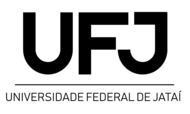
\includegraphics[width=1.5cm]{images/ufjJataiLogo.png}}

\begin{document}

	\begin{frame}
		\titlepage
	\end{frame}

	\AtBeginSection{
		\begin{frame}{Sumário}%[allowframebreaks]{Sumário}
    		\tableofcontents[currentsection]
    		%\tableofcontents[currentsection, hideothersubsections]
		\end{frame}
	}

	\begin{frame}{Plano de Aula}
		\tableofcontents
		%\tableofcontents[hideallsubsections]
	\end{frame}   

    \section{Representação, população e fitness}

\begin{frame}{Seleção: quem tem mais chance?}

    \begin{block}{Ideia}
        Indivíduos com maior fitness têm \textbf{maior probabilidade}
        de serem selecionados para reprodução.
    \end{block}

    \begin{center}
        \Large
        \[
        \boxed{\text{fitness maior}
        \quad\Longrightarrow\quad
        \text{maior chance de seleção}}
        \]
    \end{center}

    \begin{block}{Mas atenção}
        Maior fitness não significa seleção garantida.
        
        \medskip
        
        A seleção continua sendo um processo \textbf{probabilístico}.
    \end{block}

\end{frame}

\begin{frame}{Seleção por roleta}

    \begin{block}{Como funciona?}
        Cada indivíduo recebe uma porção da roleta proporcional
        ao seu fitness.
    \end{block}

    \begin{center}
        \Large
        \[
        P(i) \propto fitness(i)
        \]
    \end{center}

    \begin{block}{Consequência}
        Um indivíduo com fitness maior ocupa uma região maior
        da roleta e, portanto, possui maior probabilidade de
        ser selecionado.
    \end{block}

    \begin{center}
        \textbf{Probabilidade maior} $\neq$ \textbf{certeza}
    \end{center}

\end{frame}

\begin{frame}{Questão 014}

    \begin{block}{[Q014]}
        Uma população possui quatro indivíduos. O indivíduo $A$
        possui o maior fitness, mas os demais também ocupam partes
        da roleta.

        Após vários giros, qual comportamento é compatível com
        a seleção por roleta?
    \end{block}

    \begin{enumerate}[label=(\Alph*)]

        \item $A$ será escolhido em todos os giros, pois possui
        o maior fitness.

        \item Os quatro indivíduos terão exatamente a mesma
        chance de reprodução.

        \item $A$ terá maior probabilidade de ser escolhido,
        mas um indivíduo com fitness menor ainda poderá ser selecionado.

        \item Apenas os indivíduos que possuem o maior fitness
        participarão da próxima geração.

    \end{enumerate}

\end{frame}

\begin{frame}[shrink]{Crossover: combinar características}

    \begin{block}{Reprodução}
        Dois indivíduos selecionados podem trocar partes
        de seus cromossomos.
    \end{block}

    \begin{center}
        \large
        \[
        \underbrace{0011}_{\text{genitor 1}}
        \quad+\quad
        \underbrace{1100}_{\text{genitor 2}}
        \]
        \[
        \Downarrow
        \]
        \[
        \underbrace{0010}_{\text{filho 1}}
        \qquad
        \underbrace{1101}_{\text{filho 2}}
        \]
    \end{center}

    \begin{block}{Ideia}
        O filho combina informações provenientes de seus pais,
        aumentando as possibilidades de explorar o espaço de soluções.
    \end{block}

\end{frame}

\begin{frame}{Crossover: uma possibilidade}

    \begin{block}{Taxa de crossover}
        Mesmo depois de selecionar dois indivíduos, o cruzamento
        pode ou não acontecer.
    \end{block}

    \begin{center}
        \Large
        \[
        r \sim U(0,1)
        \]
        \[
        r \leq p_c
        \quad\Longrightarrow\quad
        \text{realiza crossover}
        \]
    \end{center}

    \begin{block}{Caso contrário}
        Os indivíduos podem ser preservados para a próxima geração.
    \end{block}

\end{frame}

\begin{frame}{Questão 015}

    \begin{block}{[Q015]}
        Dois indivíduos foram selecionados para reprodução.
        A taxa de crossover é $0{,}6$ e o sorteio associado
        ao par resultou em $0{,}8$.

        Qual interpretação está de acordo com o algoritmo?
    \end{block}

    \begin{enumerate}[label=(\Alph*)]

        \item O crossover acontece, porque os indivíduos já foram
        escolhidos pela etapa de seleção.

        \item O crossover não acontece, pois o valor sorteado
        ultrapassou a taxa definida.

        \item O crossover acontece com certeza, pois $0{,}6$
        representa a qualidade dos dois indivíduos.

        \item O par deve ser eliminado, porque um valor aleatório
        maior que a taxa indica que seus cromossomos são inválidos.

    \end{enumerate}

\end{frame}

\section{Mutação, elitismo e parada}

\begin{frame}{O problema da perda de diversidade}

    \begin{block}{Ao longo das gerações}
        A seleção favorece indivíduos com maior fitness.

        \medskip

        O crossover combina características dos indivíduos
        selecionados.
    \end{block}

    \begin{center}
        \Large
        \[
        \text{População diversa}
        \quad\longrightarrow\quad
        \text{população mais homogênea}
        \]
    \end{center}

    \begin{block}{Risco}
        Com pouca diversidade, a população pode deixar de explorar
        regiões diferentes do espaço de soluções.
    \end{block}

\end{frame}

\begin{frame}{Mutação: introduzir diversidade}

    \begin{block}{Mutação}
        Modifica aleatoriamente uma posição do cromossomo
        de acordo com uma probabilidade.
    \end{block}

    \begin{center}
        \Large
        \[
        0\,1\,1\,\boxed{0}\,1
        \quad\longrightarrow\quad
        0\,1\,1\,\boxed{1}\,1
        \]
    \end{center}

    \begin{block}{Função}
        A mutação aumenta a diversidade e pode permitir que a busca
        alcance regiões que não seriam exploradas apenas pelo crossover.
    \end{block}

\end{frame}

\begin{frame}{Taxa de mutação}

    \begin{block}{Para cada posição}
        Um valor aleatório pode ser comparado à taxa de mutação.
    \end{block}

    \begin{center}
        \Large
        \[
        r \leq p_m
        \quad\Longrightarrow\quad
        \text{mutação}
        \]
    \end{center}

    \begin{block}{Um cuidado}
        Se a taxa for muito alta, muitas posições serão alteradas,
        tornando o processo cada vez mais próximo de uma busca aleatória.
    \end{block}

\end{frame}

\begin{frame}{Questão 016}

    \begin{block}{[Q016]}
        Após várias gerações, quase todos os indivíduos de uma
        população possuem cromossomos muito semelhantes.

        O que uma taxa de mutação não nula pode proporcionar
        nesse cenário?
    \end{block}

    \begin{enumerate}[label=(\Alph*)]

        \item Garantir que o melhor indivíduo sempre permaneça
        exatamente igual na geração seguinte.

        \item Fazer com que todos os indivíduos recebam novas
        características em cada geração.

        \item Reintroduzir variações que poderiam desaparecer
        quando a população se torna excessivamente homogênea.

        \item Substituir a função de fitness por uma avaliação
        puramente aleatória das soluções.

    \end{enumerate}

\end{frame}

	\begin{frame}
		\titlepage
	\end{frame}
	
\end{document}